\documentclass{article}

\usepackage{graphicx}
\usepackage{listings}
\usepackage{url}

\title{TorConnect: An Anonymous P2P Service}
\author{James Lee\\
	\small Computer Science and Electrical Engineering\\
	\small University of Maryland, Baltimore County\\
	\small\tt jlee23@umbc.edu}
\date{\today}

\begin{document}
\maketitle
\begin{abstract}
Participating in a traditional P2P network leaves users vulnerable to identification through their public IP address.  Tor makes such analysis difficult by routing packets through multiple routers.  It also provides a mechanism to hide services in such a way that a client can still connect without either party being able to determine each other's IP address.  In this paper, I introduce TorConnect, a new P2P protocol designed to keep users anonymous by Tor hidden services.  The resulting implementation is secure and requires no setup, enabling even novice computer users to participate in an anonymous community with confidence.
\end{abstract}

\section{Introduction}
To communicate anonymously with others means that an observer is unable to identify the source, destination, and message of an intercepted packet.  Tor is a software project which anonymizes arbitrary TCP communication by routing packets through multiple nodes before reaching their destination~\cite{tor-design}.  It also provides a mechanism to hide services so that they are only accessible by a pseudonym on the Tor network.  However, users must know the pseudonym in order to establish a connection to the hidden service.  Additionally, hidden services are difficult for novice computer users to set up, requiring knowledge of private key management and TCP/IP addressing.  Because of this and the difficulty of discovering hidden services, there are no anonymous communities on the Tor network.

My intent was to make the use of Tor to communicate and share files so easy that anonymous communities can begin to grow.  To do this, I designed and implemented TorConnect, a hub-based P2P protocol similar to the popular Direct Connect service.  The protocol requires that users communicate over Tor and are identified only by pseudonyms, not IP address like typical P2P protocols.  The implementation bundles a Tor client and configures it automatically.  The client also has a graphical user interface (GUI) and a one-click installer.

\section{Motivation}
I completed this work because I want to be able to participate in a community anonymously.

Why would anyone want to remain anonymous?  Users may want to remain anonymous because they have material that is illegal or for which the distribution is illegal.  The material might just be embarrassing if not illegal.  They may also fear retribution for communicating a sensitive or offensive message.  Anonymous networks provide a great way for users to voice opinions.  They also give a voice to people who are otherwise censored by a governing body.

Typical communication on the Internet is not anonymous.  All users can be identified by their unique IP address.  Anonymous networks such as ``mixes'' as originally proposed by David Chaum in 1981 route encrypted messages through multiple nodes in a network~\cite{chaum-mix}.  As a result, no single node can discover the source, destination, and contents of a message.

Why would someone want to participate in a community?  Communities are collections of users with some shared interest.  All the users have a way to discover all the other users in the community, that way they can meet other people with a shared interest.  In communities where users are identifiable, usually by a nick name, it is possible to build a reputation with the other users, even develop friendships.  Simply put, communities are a fun and easy way of interacting with other people.

How can a community be built?  Most importantly, there must be some way for users to know the other members of the community.  Users could be known could be by nick name or pseudonym.  The users must be easy to discover.  If users can't be discovered, there is no way for someone to find someone else with whom to share their common interest.  Most users will also need some reason to join a community.  Some will expect some sort of content.  A community must also be easy to join.  If it is too difficult, users will not feel it is worth their time.  I am proposing that the ability to communicate and share files anonymously will entice users to join an anonymous community.

Users will have those abilities through the design and implementation of TorConnect, a new P2P protocol similar to Direct Connect.  They will be kept anonymous by Tor.

Why base the design off Direct Connect?  Direct Connect is known for its simplicity.  Users connect to a hub which keeps track of who is online in the community, that way new users are easily discoverable.  Hubs also facilitate searching and chatting since they serve as a single broadcast point to all users.  Also important is that having distinct hubs allow multiple communities to grow, each with special areas of interest.  A system similar to Direct Connect will give users significant incentive to join.

Why use Tor to anonymize communication?  Tor is a well-studied, mature implementation of onion-routing.  Onion-routing routes messages like Chaum's mixes, but on persistent routes, reducing latency and increasing throughput which is ideal for transferring files.  Tor is the largest active anonymity network and is the subject of academic scrutiny, the benefits of which applications built on Tor receive automatically.  Tor is unique in that it can route arbitrary TCP streams.  It provides a standard SOCKS proxy interface so most networking libraries can use Tor unmodified.  Tor also provides a mechanism to hide services so that they are only accessible by a pseudonym on the Tor network.  Clients in my system are be hidden by this mechanism and users are identified by the pseudonym that Tor provides.


\section{Previous Work}
There is a countless number of ways to build a community on the public Internet.  Very few of them guarantee anonymity and none of them are built on Tor.  Most of the work on Tor attempts to make it easier for a single user to join the network.  For example, Torbutton is an extension to Firefox which gives users a one-click way to enable access to the Tor network.  Its ease of installation and use make Tor more popular to users who wish to remain anonymous to public Internet sites.  Another popular utility, Vidalia, provides a very easy GUI for managing Tor, but provides no other means for Tor users to communicate.  That functionality must be provided by another program.

One such program which enables Tor users to communicate anonymously is TorChat~\cite{tor-chat}.  Clients are configured to act as hidden services on the Tor network, each one being assigned a unique 16 character pseudonym.  Then, a user may talk to another single user identified by his pseudonym.  TorChat is not suitable for building an anonymous community.  Due to its decentralized design the only way for users to communicate with other users is to already know them and ask them for their pseudonyms.  This make discovering new users very difficult.

However, TorChat does make setup easy on Windows.  It comes bundled with a Tor client which it configures and runs automatically.  The Linux client, on the other hand, requires users to configure Tor manually, which might restrict them from joining.  For a community to be built, it must be easy for as many people as possible to join, and that means considering all the major operating systems equally.  TorConnect, like TorChat on Windows, bundles, installs, configures, and runs Tor automatically and transparently on both Windows and Linux so that it is easy for as many users to join as possible.

TorConnect builds its community around hubs based on Direct Connect.  Direct Connect has proven community building qualities.  For example, several Direct Connect hubs have existed on the UMBC campus for years.  A student can download any Direct Connect client, type the IP address of the hub, and begin interacting with other students.  Users generally discover the address of the hub through word of mouth.  The pseudonym of an anonymous hub can be discovered the same way.

Once students have joined the hub, they have the ability to chat and share files with other students.  They can ask questions about classes, voice opinions about instructors, or talk about campus events.

Direct Connect is a very simple text-based protocol.  The ease of its implementation means that thousands of hubs like the one at UMBC have developed around the world, each with its own community serving a special interest.  Some hubs might be built around movies, others around music.

The Direct Connect protocol requires that users are identified by an IP address, though.  The IP address is revealed whenever a user establishes a connection with another user.  It can be discovered using most operating systems' network monitoring utilities, but many clients report it in the user interface.  Users of the UMBC hub quickly discovered how to associate an IP address with a residence hall, and even floor.  Members of the hub who also worked in OIT could even associate IP addresses with room numbers.

The goal of TorConnect was to take the community building qualities of Direct Connect and apply the anonymity techniques employed by TorChat to create an anonymous community.

\section{Design}
Current P2P systems are designed around IP addressing.  For example, queries to BitTorrent trackers retrieve the IP addresses of all the peers in the swarm.  Since Tor clients build circuits through multiple peers, the address of the circuit's end point, the address that the server sees, is not the true address of the initiating client.  Because of this, a whole new protocol had to be designed so that, instead of tracking IP addresses, the system tracks domain names which can hold the pseudonym of a client's hidden service.

This raises the problem of how a server can determine the hidden service pseudonym of a connecting client.  Traditional TCP servers don't have to worry about the problem; they can simply grab the source address from the IP packet with confidence that it is correct due to the protections afforded by the TCP protocol~\cite{wiki-spoofing}.  The most obvious solution is to require the client to write its pseudonym to the stream right after opening a connection.  Then the server can just read from the top.  However, there needs to be a mechanism to prevent the client from writing any random pseudonym to the stream, it \emph{must} be his own.  Thus, the TorConnect protocol requires any client to prove their identity by way of a handshake.

\subsection{Protocol}
\begin{figure}
\centering
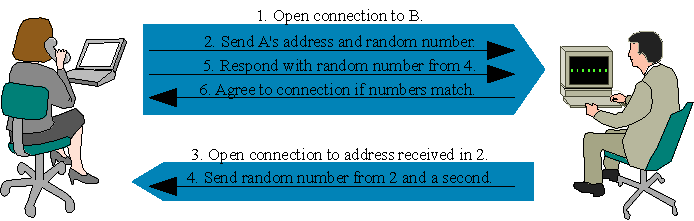
\includegraphics{handshake.pdf}
\caption{The handshaking between two anonymous parties.}
\label{fig:handshake}
\end{figure}

As pictured in figure \ref{fig:handshake}, the server verifies the pseudonym sent by the client by opening a new connection to it.  The server then sends a random integer that it should expect to receive on the original connection.  If the client sent a bogus pseudonym, the server would be unable to connect to it (because it doesn't exist) or it would connect to a client who wouldn't recognize the random number and reject the connection.

When the server is satisfied that the client is who it says it is, regular communication can continue.  In the case of TorConnect, this consists of a number of plain text commands terminated by new line characters.  A new line character is sufficient because none of the commands' arguments will ever contain a new line.

The protocol defines two communicating systems: a hub and a client.  The hub stands as a central point for directory listing, chatting, search query propagation, and results collection.  The hub never connects to other systems; it only receives connections.  A client can connect to hubs, chat, private message other users, search, and transfer files.

When the hub receives a connection from a client, it will add the client's address to a roster and announce the new arrival to the users who are already logged on.  Additionally, the hub will send a full roster to the client.  At any time, a client may also request an association with a nick name.  If it's available, that association will also be announced to all of the clients.  This way, clients can be identified by a nick name in addition to their hidden service pseudonym.  When a client wishes to disconnect, it can optionally send a message to the hub explaining the reason for the disconnection.  When the connection is closed, either intentionally or not, the hub announces the disconnection to the other users still logged on.

Users can chat with other users on their hub by sending a ``broadcast'' message to the hub, which the hub, in turn, sends to everyone connected to it.

Users can initiate searches of other users' explicitly shared files by sending the query to the hub, along with some identifying integer.  The hub will associate yet another id with the query and pass it along to all the users.  The users will perform the search and send the results back along with the query id sent by the hub.  The hub will relay the results back to the original user with their chosen query id.   That way, the user can know which search their receiving results for.

On the client side of things, users can connect to each other to chat or transfer files.  For both, the client initiates a connection to his peer, completes the handshake as required, then describes his intention: ``chat'' or ``get'' plus a file name.  Following ``chat'', whatever the user writes to the network stream is considered chat text.  The chat ends when the connection closes.  Following ``get'' plus a file name, the peer responds with the size of the file and immediately starts writing the binary data of that file to the network stream.

\subsection{Application}
\begin{figure}
\centering
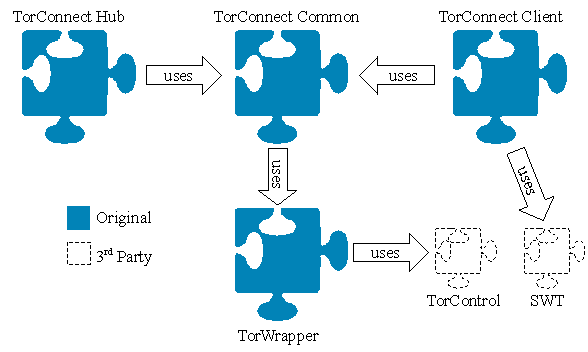
\includegraphics{architecture.pdf}
\caption{The components of TorConnect.}
\label{fig:architecture}
\end{figure}

I chose to implement TorConnect in Java.  Java is highly portable, working on multiple platforms without the need to recompile.  It is also well suited for rapid development.  The nature of the protocol led to the creation of two distinct applications, the hub and the client, which share common network-related code in a common library, all of which depend on an original Java wrapper around the Tor binary.  These relationships are depicted in figure \ref{fig:architecture}.

\subsubsection{TorWrapper}
TorConnect is highly dependent on Tor, which requires a binary proxy to be configured and running.  To meet the requirement of being easy to install and configure, I developed a Java library called TorWrapper that handles the management of all Tor processes.

First, it bundles Tor binaries for Linux and Windows with itself.  This is possible since Java libraries are simply zip files.  At runtime, a function in TorWrapper extracts the appropriate binary from itself to a temporary directory.  The binaries are statically linked so that they won't carry additional library dependencies.

Next, the newly-extracted binary is executed with a minimal set of command line options, just enough to open a control connection.  Tor provides a control connection for applications to configure and query log and status information from the running process~\cite{tor-control}.  I used a third-party library called \verb+torctl+ which exposes the control connection through a nice Java interface, rather than dealing with the low level network calls~\cite{tor-ctl}.

Finally, TorWrapper provides a function to hide a service which takes a hostname and port to be hidden, configures Tor through the control connection, and returns the hidden service pseudonym back to the calling application.  This is a typical example of how TorWrapper is used:
{ \scriptsize
\lstset{language=Java}
\begin{quote}
\begin{lstlisting}
TorWrapper torWrapper = new TorWrapper();
torWrapper.start();

ServerSocket serverSocket = new ServerSocket();
String hiddenHostname = torWrapper.hideService(
				serverSocket.getInetAddress(),
				serverSocket.getLocalPort());

// do stuff

serverSocket.close();
torWrapper.shutdown();
\end{lstlisting}
\end{quote}
}

\subsubsection{Common Utilities}
The hub and client share a lot of code relating to connections so it made sense to share it in the form of a separate library.  Among other things, it handles making outgoing connections, accepting incoming connections, and all the handshaking that occurs with new connections.  It is typically used like:
{ \scriptsize
\lstset{language=Java}
\begin{quote}
\begin{lstlisting}
IncomingConnectionListener listener =
	new IncomingConnectionListener(tor, port);
listener.addIncomingConnectionHandler(
    new IncomingConnectionHandler() {
        public void connectionReceived(Connection newConnection) {
            System.out.println("Successfully handshaked with " +
	        newConnection.getTorAddress());
	}
    }
);
listener.start();

Connection connection = new OutgoingConnection(
	new TorAddress("xxxxxxxxxxxxxxxx.onion", 5000));
connection.syncWriteLine("HI");
connection.close();

listener.shutdown();
\end{lstlisting}
\end{quote}
}

\subsubsection{TorConnect Hub}
The TorConnect Hub is a standalone, command-line program which uses the aforementioned common libraries to implement the hub protocol.  Shortly after starting, it will announce its own hidden service pseudonym on standard output.  Clients can use this address to connect to the hub.

\subsubsection{TorConnect Client}
The TorConnect Client is a standalone, graphical program which uses the aforementioned common libraries to implement the client protocol.  The GUI is implemented using the SWT toolkit, which uses the platform's native widget set so it appears like any other application on the user's computer.  It accomplished its goal of being easy to install by launching as a Java Web Start application, taking only one click to install.  The client requires no configuration out-of-the box.  Simply enter the address of a hub and it will connect.

\section{Analysis}
\subsection{Security}
For the purposes of this project, security means that it is not possible to determine the actual identity of a user in the system and that users are the pseudoanonymous identity that they claim.  Anything else is an exercise for another project.

On the protocol, there is positively no personally identifying information required for TorConnect to work.  However, neither the protocol nor the implementation prevent users from sharing personally identifying information.  A user could accidentally share files containing personal information.  Search results also return full paths, which may include system user names.  One improvement that should be made to TorConnect is to return search results containing only a substring of a shared file name plus enough additional information so that the sharer can find the file when requested, but downloaders cannot see the full path name.

Handshakes really do prevent users from spoofing their identity.  Since a server tests your identity by establishing a new outgoing connection to a client's alleged address, the only way for a client to successfully report a false address is if they also had control over the address that they claimed to be from.  But false address or not, it still represent the same (malicious) user so it doesn't pose a threat to another user's identity.  A state where a connection successfully spoofed their source may lead to errors later down the line, such as another user trying to initiate a download, but that is not a security problem.

So if you are convinced of the protocol security, then you will see that the security of the TorConnect relies on Tor.  If Tor is secure, then TorConnect is secure.

\subsection{Usability}
I feel that TorConnect meets the requirement of being so easy to use that anyone can participate in the resulting communities.  The hub takes one command to run with one argument and requires no further configuration.  The client takes one-click to install and run, and no further configuration.  Perhaps no more objective statements could be made.  I'll leave the subjective opinions to others.

Having said that, TorConnect is completely unusable.  The live Tor network is simply too unreliable to accommodate, well, anything at all.  The biggest issue is actually establishing connections to hidden services, which requires coordination of several routers, routinely fails while building circuits.  I can only attribute this to overloaded routers as evidenced by the verbose output of Tor.  Indeed, after setting up my own Tor network, hidden service connections were as fast and reliable as you'd expect.

\section{Open Problems}
The main issue preventing TorConnect from being usable is the biggest problem to be solved: how can the speed and reliability be improved?  I think that there will never be a solution as long as you are relying on volunteers on the public internet to provide the routers for the Tor network.  There just aren't enough and the ones that do exist don't provide nearly enough bandwidth for this application.

In my own testing, running my own Tor network, with my own routers made connections reliable and throughput (surprisingly) close to speeds that I would expect from other file transfer methods like SCP.  However, with such a small number of routers, traffic analysis is significantly easier.

One solution might be to require hub participants to also run a Tor router on a private Tor network.  There may also be requirements for a certain bandwidth to join the hub to prevent bottlenecks in circuits.  With only about 1,000 Tor routers running on the public Tor network, it is not inconceivable for the private TorConnect network to grow to have the same diversity, foiling traffic analysis~\cite{tor-numrouters}.

Another idea to improve connection speeds is to do away with handshakes.  Instead, use public key cryptography to authenticate a user.  A client new to the system could perform a one-time handshake with the hub and upload a newly generated public key, which the hub can associate with their pseudonym.  Then when a system receives a connection, they can check some signed string against the public key associated with the claimed address.

It would also be interesting to see a more mature P2P protocol adapted to support Tor.  Admittedly, TorConnect does not support all the features most users have come to expect from a P2P system like swarming (downloading the same file from multiple peers).

\section{Conclusions}
Before this project began, there was no way to build a community on Tor.  All of the technologies focused on simplifying or improving one-way anonymity.  Tor's built-in hidden service mechanism enables a sort of two-way anonymity.  With the addition of handshaking, it became possible for both parties in an anonymous connection to know each other's pseudoanonymous identities.  Even still, you won't be connecting to many hidden services if you can't discover them, thus the hub.  The hub keeps track of anonymous community participants.  Once you've discovered another person's hidden service pseudonym, you can effectively communicate in any way you want.  I have proposed that chatting and file-sharing are activities that would entice users to join the network.  I have implemented these systems in TorConnect, which successfully proved my concept.

\bibliographystyle{unsrturl}
\bibliography{report}

\appendix
\newpage
\section{Protocol Documentation}
\label{app:protocol}
\subsection{Overview}
The following describes the communication between systems in TorConnect, a peer-to-peer (P2P) system built on Tor.  This protocol will consist of simple plain text commands sent between clients and hubs.  The hub stands as a central point for directory listing, chatting, search query propagation, and results collection.  A client must have the ability to connect to a single hub, chat, private message, search, display file lists, and transfer files.

All connections must be made through Tor and every client and hub must have some hidden service identified by an onion address with which they can be contacted.  Clients and hubs must know their own address.

\subsection{Handshake}
All connections, whether from client-to-hub or client-to-client, must begin with a handshake to prove to the receiver that the initiator is who he says he is.

\begin{description}
\item[A] \verb+YO <A's address> <rand1>+
\item[B] \verb+SUP <rand1> <rand2>+
\item[A] \verb+NOTMUCH <rand2>+
\item[B] \verb+<COOL|NOTCOOL> [<message>]+
\end{description}

A opens a connection to B sending his known onion address and a random integer \verb+rand1+.  B opens a new connection to A's address sending the original \verb+rand1+ plus another random integer \verb+rand2+.  Finally A responds on the original connection associated with \verb+rand1+ sending \verb+rand2+ back to B.  Now B knows that A's address is valid and communication can continue on the first connection.  The second can be disconnected.

If at any point these messages should not pass as expected, the connection should be closed.  If a handshake is not successful within a minute, the connection should be closed.

\subsection{Client-to-hub Communication}
Once a client connects to a hub, and a handshake is completed successfully, the hub will know the client's address and communication can continue using the following messages.

\subsubsection{Nick Name}
A client can optionally have a nickname for their complicated onion address.  It's only use is in the user interface.

\begin{description}
\item[Client] \verb+NICK <nick>+
\item[Hub] \verb+<COOL|NOTCOOL> [<message>]+
\end{description}

The hub should note the correspondence between onion address and nick name and announce the nick name to all the clients.

\subsubsection{Broadcast Message}
Clients should be able to broadcast messages to all the other clients connected through the hub.  This can result in a sort of chat.

\begin{description}
\item[Client] \verb+BROADCAST <message>+
\item[Hub] \verb+<COOL|NOTCOOL> [<message>]+
\end{description}

\subsubsection{Search}
Clients should be able to initiate search requests through the hub.

\begin{description}
\item[Client] \verb+SEARCH <id> <regex>+
\item[Hub] \verb+<COOL|NOTCOOL> [<message>]+
\end{description}

\verb+id+ is a unique integer specified by the client to identify a particular search query.  This will be important to know what query results belong to.  The \verb+regex+ regular expression must be Java compatible.

\subsubsection{Search Results}
\begin{description}
\item[Client] \verb+SEARCHRESULT <id> <size> <filename>+
\item[Hub] \verb+<COOL|NOTCOOL> [<message>]+
\end{description}

A client should be able to return search results for a query back to the hub.  For each hit, this message should be sent.  \verb+id+ is the same \verb+id+ from the original query.

\subsubsection{Close Search}
\begin{description}
\item[Client] \verb+CLOSESEARCH <id>+
\item[Hub] \verb+<COOL|NOTCOOL> [<message>]+
\end{description}

This instructs the hub to stop relaying search results for the original query with the id \verb+id+.

\subsubsection{Disconnection}
\begin{description}
\item[Client] \verb+DISCONNECT [<reason>]+
\item[Hub] \verb+<COOL|NOTCOOL> [<message>]+
\end{description}

This message will be sent to the hub just before the user disconnects.

\subsection{Hub-to-client Communication}

\subsubsection{Client Connection}
\begin{description}
\item[Hub] \verb+CONNECT <address>+
\end{description}

This message gets sent to all logged in users when a new user logs on to the hub.

\subsubsection{Client Nick Change}
\begin{description}
\item[Hub] \verb+NICK <address> <nick>+
\end{description}

This message gets sent to all logged in users when a user sends a \verb+NICK+ message to the hub.

\subsubsection{Broadcast Message}
\begin{description}
\item[Hub] \verb+BROADCAST <address> <message>+
\end{description}

This message gets sent to all logged in users when a user sends a \verb+BROADCAST+ message to the hub.

\subsubsection{Search}
\begin{description}
\item[Hub] \verb+SEARCH <id> <regex>+
\end{description}

This is the relay message for client search requests.  The \verb+id+ is a unique integer so that a hub knows which query search results belong to when they arrive.

\subsubsection{Search Results}
\begin{description}
\item[Hub] \verb+SEARCHRESULT <id> <address> <size> <filename>+
\end{description}

This message gets sent to the user belonging to a query's \verb+id+ when it receives a \verb+SEARCHRESULT+ message from another user.

\subsubsection{Disconnection}
\begin{description}
\item[Hub] \verb+DISCONNECT <address> [<reason>]+
\end{description}

This message get sent to all logged in users when a user sends a \verb+DISCONNECT+ message to the hub.

\subsection{Client-to-client Communication}

\subsubsection{Chat}
\begin{description}
\item[A] \verb+CHAT+
\end{description}

Any messages following this will be considered part of the chat.

\subsubsection{Get File}
\begin{description}
\item[A] \verb+GET <filename>+
\item[B] \verb+SIZE <bytes>+
\end{description}

When a client receives this message, they should send the binary data contained in \verb+filename+ (if shared) after sending its size.

\subsection{Handling Errors}
Should a system receive an invalid message, they may send a \verb+NOTCOOL+ message to inform the other system of the error.  They may also choose to disconnect if it seems more appropriate.  Any system should be able to handle disconnection at any time.

\newpage
\section{Implementation Documentation}
My implementation of TorConnect lives in Subversion at \url{http://thestaticvoid.org/torconnect/}.  It can be checked out and built on the command line:

\begin{verbatim}
$ svn co http://thestaticvoid.org/torconnect/trunk torconnect
$ cd torconnect
$ ./run-hub.sh
\end{verbatim}

The codebase is also ready to import into Eclipse.  I recommend this for running and testing the GUI.  Once imported into Eclipse, the class \texttt{org\-.the\-static\-void\-.tor\-connect\-.client\-.Client} can be run as an SWT application.

\end{document}
